% Options for packages loaded elsewhere
\PassOptionsToPackage{unicode}{hyperref}
\PassOptionsToPackage{hyphens}{url}
%
\documentclass[
  ignorenonframetext,
]{beamer}
\usepackage{pgfpages}
\setbeamertemplate{caption}[numbered]
\setbeamertemplate{caption label separator}{: }
\setbeamercolor{caption name}{fg=normal text.fg}
\beamertemplatenavigationsymbolsempty
% Prevent slide breaks in the middle of a paragraph
\widowpenalties 1 10000
\raggedbottom
\setbeamertemplate{part page}{
  \centering
  \begin{beamercolorbox}[sep=16pt,center]{part title}
    \usebeamerfont{part title}\insertpart\par
  \end{beamercolorbox}
}
\setbeamertemplate{section page}{
  \centering
  \begin{beamercolorbox}[sep=12pt,center]{part title}
    \usebeamerfont{section title}\insertsection\par
  \end{beamercolorbox}
}
\setbeamertemplate{subsection page}{
  \centering
  \begin{beamercolorbox}[sep=8pt,center]{part title}
    \usebeamerfont{subsection title}\insertsubsection\par
  \end{beamercolorbox}
}
\AtBeginPart{
  \frame{\partpage}
}
\AtBeginSection{
  \ifbibliography
  \else
    \frame{\sectionpage}
  \fi
}
\AtBeginSubsection{
  \frame{\subsectionpage}
}
\usepackage{amsmath,amssymb}
\usepackage{lmodern}
\usepackage{iftex}
\ifPDFTeX
  \usepackage[T1]{fontenc}
  \usepackage[utf8]{inputenc}
  \usepackage{textcomp} % provide euro and other symbols
\else % if luatex or xetex
  \usepackage{unicode-math}
  \defaultfontfeatures{Scale=MatchLowercase}
  \defaultfontfeatures[\rmfamily]{Ligatures=TeX,Scale=1}
\fi
% Use upquote if available, for straight quotes in verbatim environments
\IfFileExists{upquote.sty}{\usepackage{upquote}}{}
\IfFileExists{microtype.sty}{% use microtype if available
  \usepackage[]{microtype}
  \UseMicrotypeSet[protrusion]{basicmath} % disable protrusion for tt fonts
}{}
\makeatletter
\@ifundefined{KOMAClassName}{% if non-KOMA class
  \IfFileExists{parskip.sty}{%
    \usepackage{parskip}
  }{% else
    \setlength{\parindent}{0pt}
    \setlength{\parskip}{6pt plus 2pt minus 1pt}}
}{% if KOMA class
  \KOMAoptions{parskip=half}}
\makeatother
\usepackage{xcolor}
\IfFileExists{xurl.sty}{\usepackage{xurl}}{} % add URL line breaks if available
\IfFileExists{bookmark.sty}{\usepackage{bookmark}}{\usepackage{hyperref}}
\hypersetup{
  pdftitle={A 56 year old woman with progressive weakness},
  pdfauthor={David Wilkins},
  hidelinks,
  pdfcreator={LaTeX via pandoc}}
\urlstyle{same} % disable monospaced font for URLs
\newif\ifbibliography
\usepackage{longtable,booktabs,array}
\usepackage{calc} % for calculating minipage widths
\usepackage{caption}
% Make caption package work with longtable
\makeatletter
\def\fnum@table{\tablename~\thetable}
\makeatother
\usepackage{graphicx}
\makeatletter
\def\maxwidth{\ifdim\Gin@nat@width>\linewidth\linewidth\else\Gin@nat@width\fi}
\def\maxheight{\ifdim\Gin@nat@height>\textheight\textheight\else\Gin@nat@height\fi}
\makeatother
% Scale images if necessary, so that they will not overflow the page
% margins by default, and it is still possible to overwrite the defaults
% using explicit options in \includegraphics[width, height, ...]{}
\setkeys{Gin}{width=\maxwidth,height=\maxheight,keepaspectratio}
% Set default figure placement to htbp
\makeatletter
\def\fps@figure{htbp}
\makeatother
\setlength{\emergencystretch}{3em} % prevent overfull lines
\providecommand{\tightlist}{%
  \setlength{\itemsep}{0pt}\setlength{\parskip}{0pt}}
\setcounter{secnumdepth}{-\maxdimen} % remove section numbering
\ifLuaTeX
  \usepackage{selnolig}  % disable illegal ligatures
\fi

\title{A 56 year old woman with progressive weakness}
\author{David Wilkins}
\date{29 April 2021}
\institute{Gen Med 008}

\begin{document}
\frame{\titlepage}

\begin{frame}{EC}
\protect\hypertarget{ec}{}
\begin{itemize}
\tightlist
\item
  56 year old woman
\item
  Lives alone, not currently employed
\item
  Previously fully independent in ADLs and mobility (until September
  2020)
\end{itemize}
\end{frame}

\begin{frame}{Presenting complaint}
\protect\hypertarget{presenting-complaint}{}
\begin{itemize}
\tightlist
\item
  Presented to the QEH Emergency Department in April 2021
\end{itemize}

--

\begin{itemize}
\tightlist
\item
  Progressive weakness since September 2020

  \begin{itemize}
  \tightlist
  \item
    Initially in thighs then later in shoulders and arms
  \item
    Associated with cramping and shooting pains in same areas, often
    after walking
  \item
    Unable to stand for long periods, legs giving way while standing,
    needs to use her hands to swing her legs out of bed in the morning
  \item
    Can no longer access high shelves
  \item
    Occasional tingling in arms and legs
  \end{itemize}
\end{itemize}

--

\begin{itemize}
\tightlist
\item
  Constant dizziness since around November 2020

  \begin{itemize}
  \tightlist
  \item
    Nil vertigo, nil ear pain, nil hearing changes
  \end{itemize}
\end{itemize}

--

\begin{itemize}
\tightlist
\item
  Weight loss of 10 kg since around November 2020

  \begin{itemize}
  \tightlist
  \item
    Reduction in appetite
  \item
    Difficulty in swallowing
  \end{itemize}
\end{itemize}

--

\begin{itemize}
\tightlist
\item
  Low mood
\end{itemize}
\end{frame}

\begin{frame}{Presenting complaint}
\protect\hypertarget{presenting-complaint-1}{}
\begin{itemize}
\tightlist
\item
  Nil focal infective signs or symptoms
\item
  Nil other systemic symptoms
\item
  Nil sick contacts
\item
  Nil recent medication changes
\item
  Previous MRI, CT head, full body PET by GP unremarkable
\end{itemize}
\end{frame}

\begin{frame}{Past medical history}
\protect\hypertarget{past-medical-history}{}
\begin{itemize}
\tightlist
\item
  GORD
\item
  Asthma
\item
  Raised peroxidase antibodies but no formal diagnosis of Hashimoto's
  thyroiditis
\item
  Right shoulder bursitis
\item
  Chronic neck and back pain with degenerative disc disease
\item
  Anxiety
\item
  Depression
\item
  Insomnia
\item
  Left ovarian cystectomy
\end{itemize}
\end{frame}

\begin{frame}{Regular medications}
\protect\hypertarget{regular-medications}{}
\begin{itemize}
\item
  amitriptyline 25 mg nocte
\item
  meloxicam 7.5 mg nocte PRN
\item
  paracetamol 500 mg + codeine 30 mg nocte PRN
\item
  nitrazepam 5 mg nocte
\item
  paracetamol 1 g QID
\item
  budesonide 200 μg + formoterol 6 μg/dose MDI 2 puffs BD PRN
\item
  salbutamol 100 μg/dose MDI 4--6 puffs q4h PRN
\item
  esomeprazole 20 mg daily
\item
  cholecalciferol 1000 units mane
\item
  estradiol pessary 10 μg Monday/Wednesday/Friday
\item ~
  \hypertarget{estradiol-1-mg-estradiol-dydrogesterone-10-mg-mane}{%
  \subsection{estradiol 1 mg + estradiol-dydrogesterone 10 mg
  mane}\label{estradiol-1-mg-estradiol-dydrogesterone-10-mg-mane}}
\end{itemize}
\end{frame}

\begin{frame}{Substances}
\protect\hypertarget{substances}{}
\begin{itemize}
\tightlist
\item
  Current pack a day smoker with 40 pack year history (though had been
  `vaping' for three months until about a week before presentation)
\item
  Occasional alcohol
\item
  Denies illicit drugs
\end{itemize}
\end{frame}

\begin{frame}{Family history}
\protect\hypertarget{family-history}{}
\begin{itemize}
\tightlist
\item
  Rheumatoid arthritis (sister only)
\item
  Thyroid disease (mother and sister)
\item
  Nil family history of malignancy
\end{itemize}
\end{frame}

\begin{frame}{Examination}
\protect\hypertarget{examination}{}
\begin{itemize}
\item
  \textbf{Vitals}: BP 131/100, HR 113, SpO2 97\% on RA, afebrile
\item
  \textbf{Respiratory}: Chest clear
\item
  \textbf{Cardiovascular}: Heart sounds dual with no murmur,
  peripherally warm and well perfused, nil peripheral oedema, calves
  soft and non-tender
\item
  \textbf{Abdomen}: Soft and non-tender, bowel sounds present
\item ~
  \hypertarget{skin-pityriasis-versicolor-across-upper-back-nil-other-rash}{%
  \subsection{\texorpdfstring{\textbf{Skin}: pityriasis versicolor
  across upper back, nil other
  rash}{Skin: pityriasis versicolor across upper back, nil other rash}}\label{skin-pityriasis-versicolor-across-upper-back-nil-other-rash}}
\end{itemize}
\end{frame}

\begin{frame}{Examination}
\protect\hypertarget{examination-1}{}
\begin{itemize}
\tightlist
\item
  \textbf{Bulk}: muscle wasting in bilateral proximal arms
\item
  \textbf{Tone}: normal in upper and lower limbs bilaterally
\end{itemize}

.pull-left{[} \textbar{} \textbf{Power} \textbar{} \textbf{Right}
\textbar{} \textbf{Left} \textbar{}
\textbar----\textbar-------\textbar------\textbar{} \textbar{} Shoulder
abduction \textbar{} 4/5 \textbar{} 4/5 \textbar{} \textbar{} Shoulder
adduction \textbar{} 4/5 \textbar{} 4/5\textbar{} \textbar{} Elbow
flexion \textbar{} 4/5 \textbar{} 4/5\textbar{} \textbar{} Elbow
extension \textbar{} 4/5 \textbar{} 4/5\textbar{} \textbar{} Wrist
flexion \textbar{} 5/5 \textbar{} 5/5\textbar{} \textbar{} Wrist
extension \textbar{} 5/5 \textbar{} 5/5\textbar{} \textbar{} Finger
abduction \textbar{} 5/5 \textbar{} 5/5\textbar{} \textbar{} Grip
strength \textbar{} 5/5 \textbar{} 5/5\textbar{]}

.pull-right{[} \textbar{} \textbf{Power} \textbar{} \textbf{Right}
\textbar{} \textbf{Left} \textbar{}
\textbar----\textbar-------\textbar------\textbar{} \textbar{} Hip
flexion \textbar{} 3/5 \textbar{} 3/5\textbar{} \textbar{} Hip extension
\textbar{} 3/5 \textbar{} 3/5\textbar{} \textbar{} Knee flexion
\textbar{} 4/5 \textbar{} 4/5\textbar{} \textbar{} Knee extension
\textbar{} 4/5 \textbar{} 4/5\textbar{} \textbar{} Ankle dorsiflexion
\textbar{} 5/5 \textbar{} 5/5\textbar{} \textbar{} Ankle plantarflexion
\textbar{} 5/5 \textbar{} 5/5\textbar{} \textbar{} Great toe
dorsiflexion \textbar{} 5/5 \textbar{} 5/5\textbar{} \textbar{} Great
toe plantarflexion \textbar{} 5/5 \textbar{} 5/5\textbar{]}

~~~ .center{[}No improvement in power post exercise{]}
\end{frame}

\begin{frame}{Examination}
\protect\hypertarget{examination-2}{}
\begin{itemize}
\tightlist
\item
  \textbf{Reflexes}:

  \begin{itemize}
  \tightlist
  \item
    Absent biceps, triceps, brachioradialis, knee jerk, ankle jerk
    reflexes bilaterally
  \item
    Downgoing plantars bilaterally
  \end{itemize}
\item
  \textbf{Coordination}: normal finger-nose test, nil
  dysdiadochokinesia, normal heel-shin test
\item
  \textbf{Sensation}:

  \begin{itemize}
  \tightlist
  \item
    Intact light touch to upper and lower limbs bilaterally
  \item
    Intact pinprick to upper and lower limbs bilaterally
  \item
    Proprioception intact in upper limbs, absent distal to knees on
    bilateral lower limbs
  \end{itemize}
\item
  \textbf{Cranial nerves} II--XII unremarkable:

  \begin{itemize}
  \tightlist
  \item
    2--3 beats non-sustained nystagmus on lateral gaze
  \item
    Minor fatiguability of upward gaze
  \item
    Otherwise normal eye movements with nil diplopia
  \item
    5/5 power to sternocleidomastoid and shoulder elevation bilaterally
  \end{itemize}
\item
  \textbf{Gait}: mildly ataxic
\item
  Normal head impulse test
\end{itemize}
\end{frame}

\begin{frame}{Initial investigations}
\protect\hypertarget{initial-investigations}{}
\begin{itemize}
\tightlist
\item
  EUC: Na 140, K+ 4.5, urea 2.3, Cr 39, eGFR \textgreater{} 90
\item
  Albumin 41, bilirubin 4, LFTs unremarkable
\item
  CK 38
\item
  CBE: Hb 137, WCC 9.29, platelets 421
\item
  TFTs, Vitamin D, B12, iron studies unremarkable
\end{itemize}
\end{frame}

\begin{frame}{Differentials}
\protect\hypertarget{differentials}{}
\begin{itemize}
\tightlist
\item
  LMN (CIDP/Guillain--Barré/Miller Fisher syndrome)
\item
  Limb-girdle muscular dystrophy
\item
  Malignancy with paraneoplastic syndrome
\item
  Metabolic myopathy
\item
  Polymyalgia rheumatica
\item
  Myasthenia gravis, Lambert-Eaton myasthenic syndrome
\end{itemize}
\end{frame}

\begin{frame}{Electromyography and nerve conduction studies}
\protect\hypertarget{electromyography-and-nerve-conduction-studies}{}
\begin{quote}
The sensory responses in the upper and lower limbs are all robust and
well within normal limits. Lower limb motor responses are small and
distal motor latencies are moderately prolonged, though the feet are
cool. There is mild slowing of motor conduction velocity in the right
common peroneal nerve. Both tibial F wave responses are within normal
latency for her height, though the right was less persistent than
expected (30\%) and some A waves were seen. \textbf{The motor responses
in the upper limbs were very small and this was out of keeping with the
power on physical examination. This was repeated multiple times with no
technical cause identified. The motor response amplitude dramatically
increased (\textgreater{} 300\%) after 10 seconds of exercise.} The
phenomenon was observed in both the median-aPB and ulnar-ADM studies.
\end{quote}

\begin{longtable}[]{@{}
  >{\raggedright\arraybackslash}p{(\columnwidth - 0\tabcolsep) * \real{0.06}}@{}}
\toprule
\endhead
class: inverse \\
\# Normal physiology of NMJ \\
.center{[}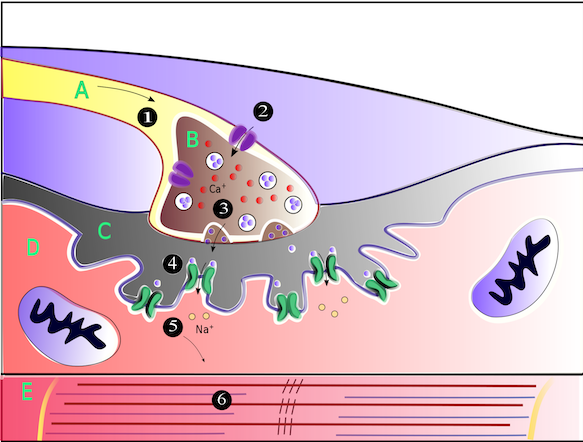
\includegraphics{nmj.png}{]} \\
.footnote{[}Author: Elliejellybelly1 • CC-BY-SA-4.0
\url{https://creativecommons.org/licenses/by-sa/4.0/deed.en}{]} \\
\bottomrule
\end{longtable}
\end{frame}

\begin{frame}{Pathophysiology of LEMS}
\protect\hypertarget{pathophysiology-of-lems}{}
\begin{itemize}
\tightlist
\item
  Autoantibodies directed against pre-synaptic voltage-gated calcium
  channels (VGCCs)

  \begin{itemize}
  \tightlist
  \item
    Ten subtypes of VGCCs in humans, defined by α1 subunit
  \item
    P/Q type (named for Purkinje neurones and cerebellar granule cells)
    comprise \textgreater95\% of VGCCs at NMJ and are major autoantibody
    target in LEMS
  \item
    Autoantibody activity against P/Q type VGCCs in the cerebellum may
    explain ataxia/loss of coordination
  \end{itemize}
\item
  SCLC cell lines have been shown to express P/Q type VGCCs (as well as
  many other components of the NMJ including ACh receptor subunits)1
\item
  Non-paraneoplastic LEMS is poorly understood, however is associated
  with other autoimmune conditions including T1DM and immune-mediated
  thyroid disease
\end{itemize}

.footnote{[} {[}1{]} Benatar M, Blaes F, Johnston I, et al.~Presynaptic
neuronal antigens expressed by a small cell lung carcinoma cell line.
Journal of Neuroimmunology. 2001;(113):153-162.{]}
\end{frame}

\begin{frame}{Epidemiology}
\protect\hypertarget{epidemiology}{}
\begin{itemize}
\tightlist
\item
  Estimates of point prevalence range from 2.3/million (region of the
  Netherlands1) to 2.6/million (US military veteran population2)
\item
  Typically diagnosed in middle age (58 ± 141)
\item
  May be somewhat more prevalent in males
\item
  At least 50\% of LEMS cases are associated with malignancy
\item
  Approximately 3\% of SCLC patients will develop LEMS (n = 63)3
\end{itemize}

.footnote{[} {[}1{]} Wirtz PW, Nijnuis MG, Sotodeh M, et al.~The
epidemiology of myasthenia gravis, Lambert-Eaton myasthenic syndrome and
their associated tumours in the northern part of the province of South
Holland. J Neurol. 2003;250(6):698-70

{[}2{]} Abenroth DC, Smith AG, Greenlee JE, Austin SD, Clardy SL.
Lambert-Eaton myasthenic syndrome: Epidemiology and therapeutic response
in the national veterans affairs population. Muscle Nerve.
2017;56(3):421-426

{[}3{]} Payne M, Bradbury P, Lang B, et al.~Prospective study into the
incidence of Lambert Eaton myasthenic syndrome in small cell lung
cancer. J Thorac Oncol. 2010;5(1):34-38. {]}
\end{frame}

\begin{frame}{Clinical features}
\protect\hypertarget{clinical-features}{}
\begin{itemize}
\tightlist
\item
  Progressive proximal muscle weakness

  \begin{itemize}
  \tightlist
  \item
    Lower limbs \textgreater{} upper limbs
  \item
    Often associated with myalgia
  \item
    Functional decline \textgreater{} loss of power
  \item
    Marked reduction or absence of deep tendon reflexes
  \item
    Paraneoplastic form typically has more rapid progression with more
    widespread weakness
  \item
    Can progress to diaphragmatic involvement and respiratory failure
  \end{itemize}
\item
  Post-exercise recovery in power and deep tendon reflexes
\item
  Autonomic dysfunction

  \begin{itemize}
  \tightlist
  \item
    Dry mouth and erectile dysfunction most common reported symptoms;
    constipation, diarrhoea, postural symptoms, dry eyes, and changes to
    sweating have also been reported1
  \item
    Pupils may be sluggish .footnote{[} {[}1{]} O'Suilleabhain P, Low
    PA, Lennon VA. Autonomic dysfunction in the Lambert-Eaton myasthenic
    syndrome: Serologic and clinical correlates. Neurology.
    1998;50(1):88-93.{]}
  \end{itemize}
\end{itemize}
\end{frame}

\begin{frame}{Clinical features}
\protect\hypertarget{clinical-features-1}{}
\begin{itemize}
\tightlist
\item
  Cranial nerve symptoms less common
\item
  Typically bulbar symptoms
\item
  Ocular signs (ptosis, diplopia) much rarer than in MG
\end{itemize}
\end{frame}

\begin{frame}{Diagnosis}
\protect\hypertarget{diagnosis}{}
\begin{itemize}
\tightlist
\item
  EMG/NCS

  \begin{itemize}
  \tightlist
  \item
    Repetitive nerve stimulation (RNS) e.g.~20 Hz for 10 seconds →
    ~increase in CMAP \textgreater{} 100\% (`postactivation
    facilitation')
  \item
    Latency and velocity are typically normal
  \end{itemize}
\item
  P/Q type VGCC autoantibody radioimmunoassay

  \begin{itemize}
  \tightlist
  \item
    85--95\% sensitivity however low specificity; present at varying
    levels in other conditions including malignancies, paraneoplastic
    syndromes and MG
  \end{itemize}
\end{itemize}
\end{frame}

\begin{frame}{Treatment}
\protect\hypertarget{treatment}{}
\begin{itemize}
\item
  Indication for treatment is based on functional impairment; watch and
  wait may be appropriate for patients with mild symptoms
\item
  Amifampridine

  \begin{itemize}
  \tightlist
  \item
    Presynaptic potassium channel blockade
  \item
    Prolongs presynaptic depolarisation → increased calcium entry
  \item
    TGA Special Access Scheme
  \item
    Mild adverse effects (headache, nausea, abdominal pain, diarrhoea),
    can cause seizures at high doses
  \end{itemize}
\item
  Pyridostigmine

  \begin{itemize}
  \tightlist
  \item
    Of limited benefit
  \end{itemize}
\item
  Guanadine

  \begin{itemize}
  \tightlist
  \item
    Narrow therapeutic window - nephrotoxicity, bone marrow suppression
  \end{itemize}
\item
  IVIG, steroids, immunosuppression, plasmapheresis
\end{itemize}
\end{frame}

\begin{frame}{Prognosis}
\protect\hypertarget{prognosis}{}
\begin{itemize}
\tightlist
\item
  In paraneoplastic LEMS, malignancy is usually life-limiting factor

  \begin{itemize}
  \tightlist
  \item
    SCLC typically diagnosed in patients with LEMS ten years earlier
    than those without 1
  \item
    Patients with SCLC and LEMS typically have significantly longer
    survival than patients without (24 months, 95\% CI 7--41 vs 7
    months, 95\% CI 5--9, n = 1482)
  \end{itemize}
\item
  Life expectancy in non-paraneoplastic LEMS is unchanged
\end{itemize}

.footnote{[} {[}1{]} Wirtz PW, Nijnuis MG, Sotodeh M, et al.~The
epidemiology of myasthenia gravis, Lambert-Eaton myasthenic syndrome and
their associated tumours in the northern part of the province of South
Holland. J Neurol. 2003;250(6):698-701. {[}2{]} Wirtz PW, Lang B, Graus
F, et al.~P/Q-type calcium channel antibodies, Lambert-Eaton myasthenic
syndrome and survival in small cell lung cancer. Journal of
Neuroimmunology. 2005;164(1-2):161-165.{]} ---
\end{frame}

\begin{frame}{EC}
\protect\hypertarget{ec-1}{}
\begin{itemize}
\tightlist
\item
  Subsequent investigation with CT and PET found FDG-avid paraortic
  lymph node
\item
  Biopsy demonstrated small cell carcinoma
\item
  Commenced on amifampridine
\item
  Commenced on cisplatin and etoposide chemotherapy, has been referred
  for radiotherapy
\end{itemize}
\end{frame}

\end{document}
